\section{Kriechen}
    \subsection{Definiton}
        \begin{itemize}
            \item Inelastische Dehnunen
            \item Für Sekundärkriechen: $\dot{\varepsilon}_{cr} = f(T,\sigma)$;\\$\sigma = \textrm{const.} \Rightarrow \dot{\varepsilon}_{cr}= \textrm{const.}$
        \end{itemize}
        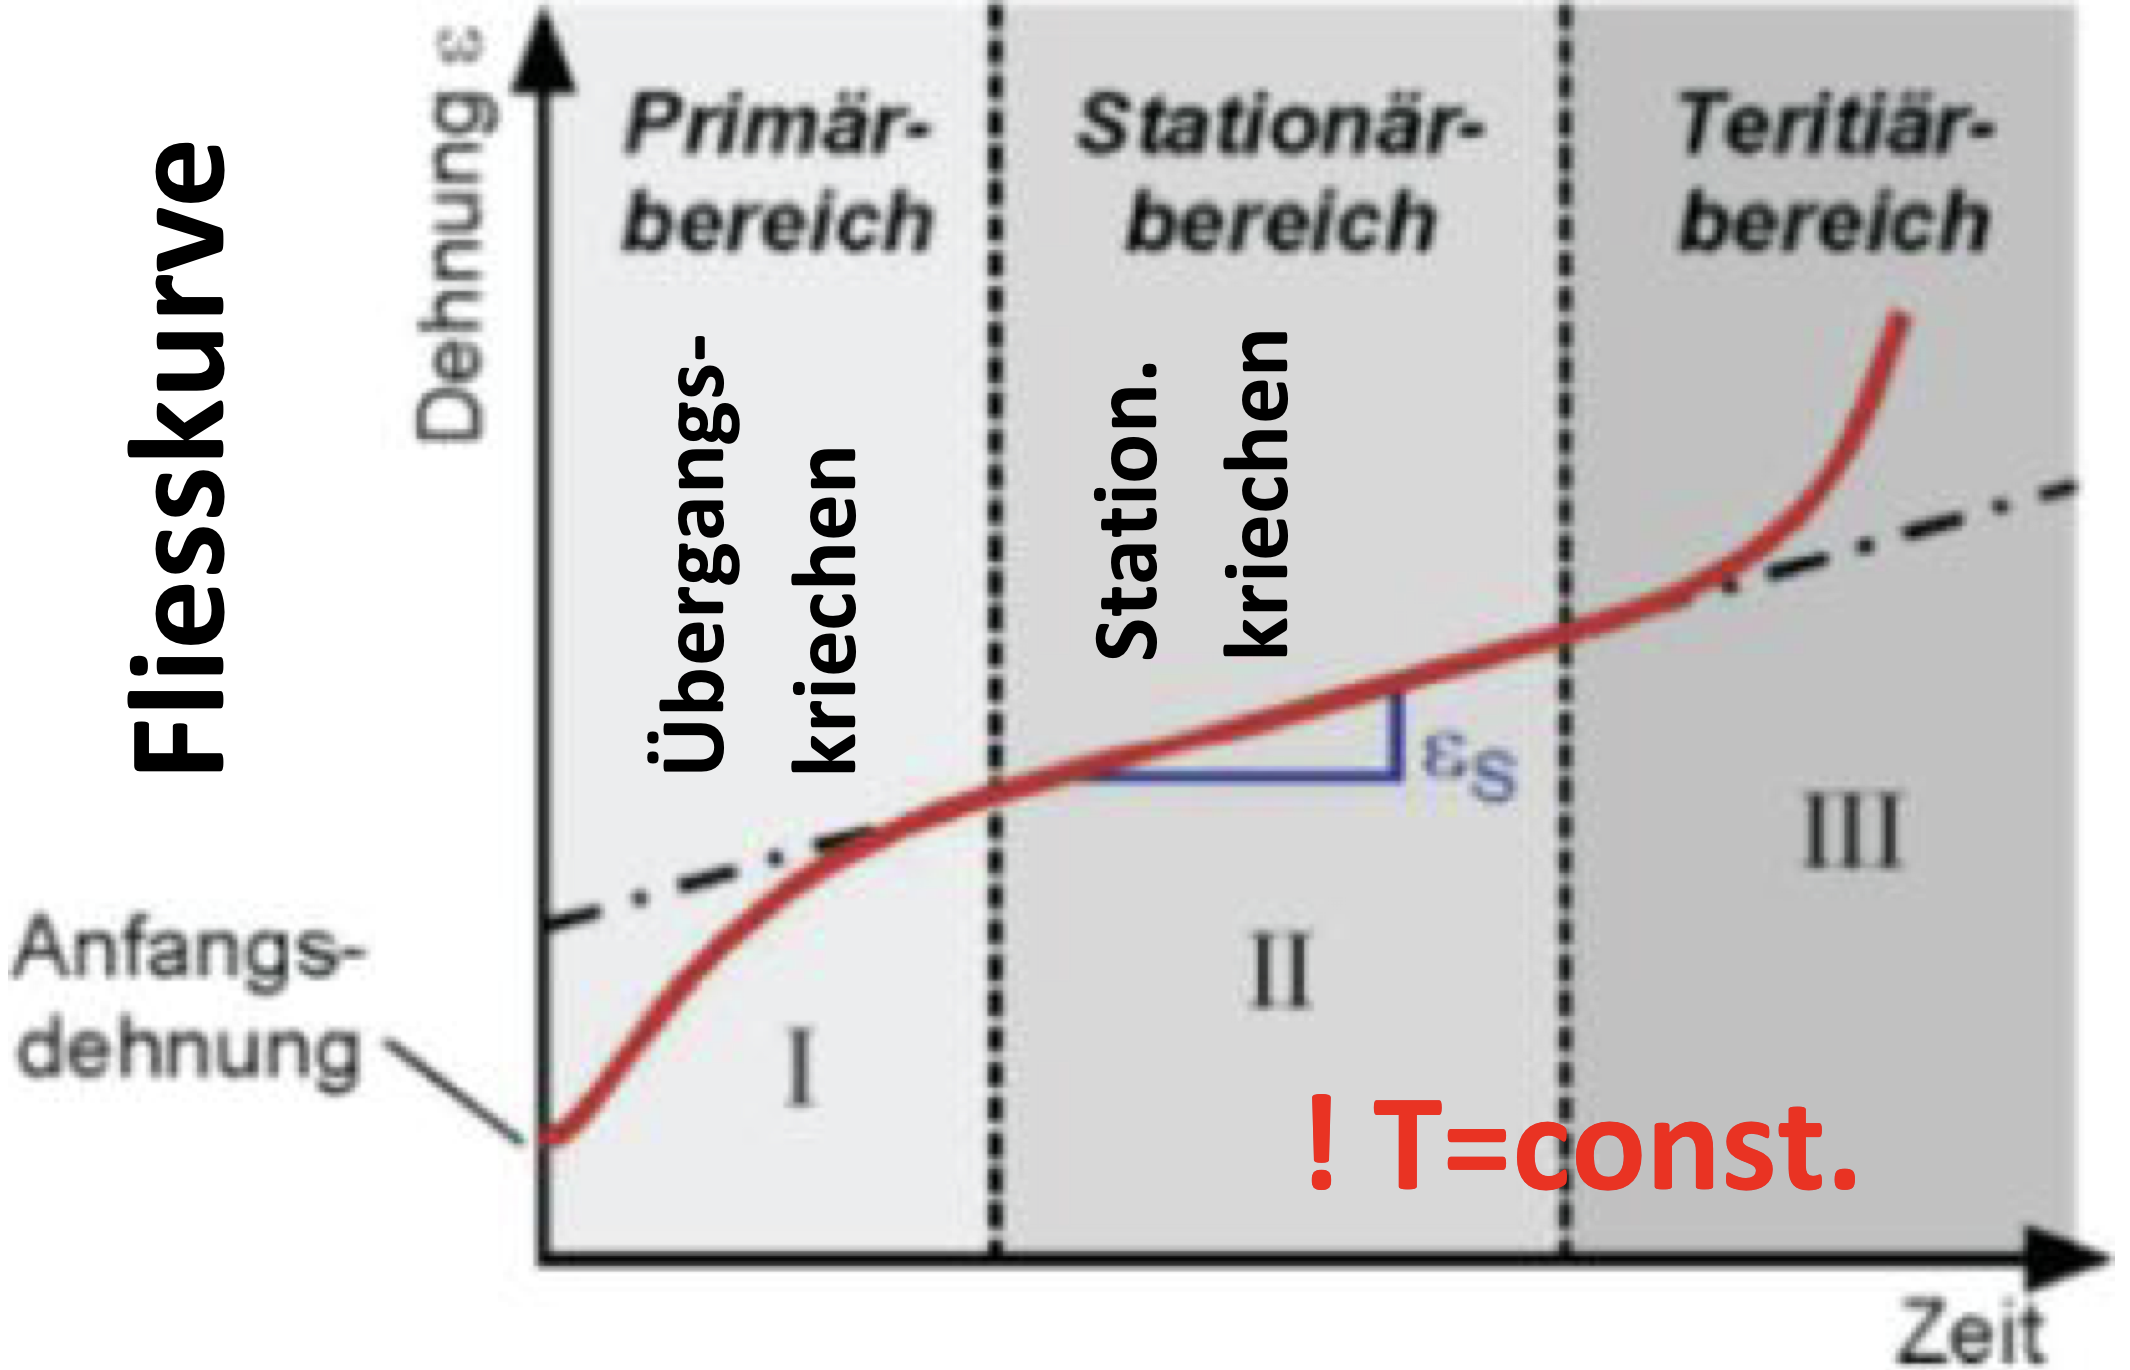
\includegraphics[width=0.45\linewidth]{08/Kriechkurve1.png}
        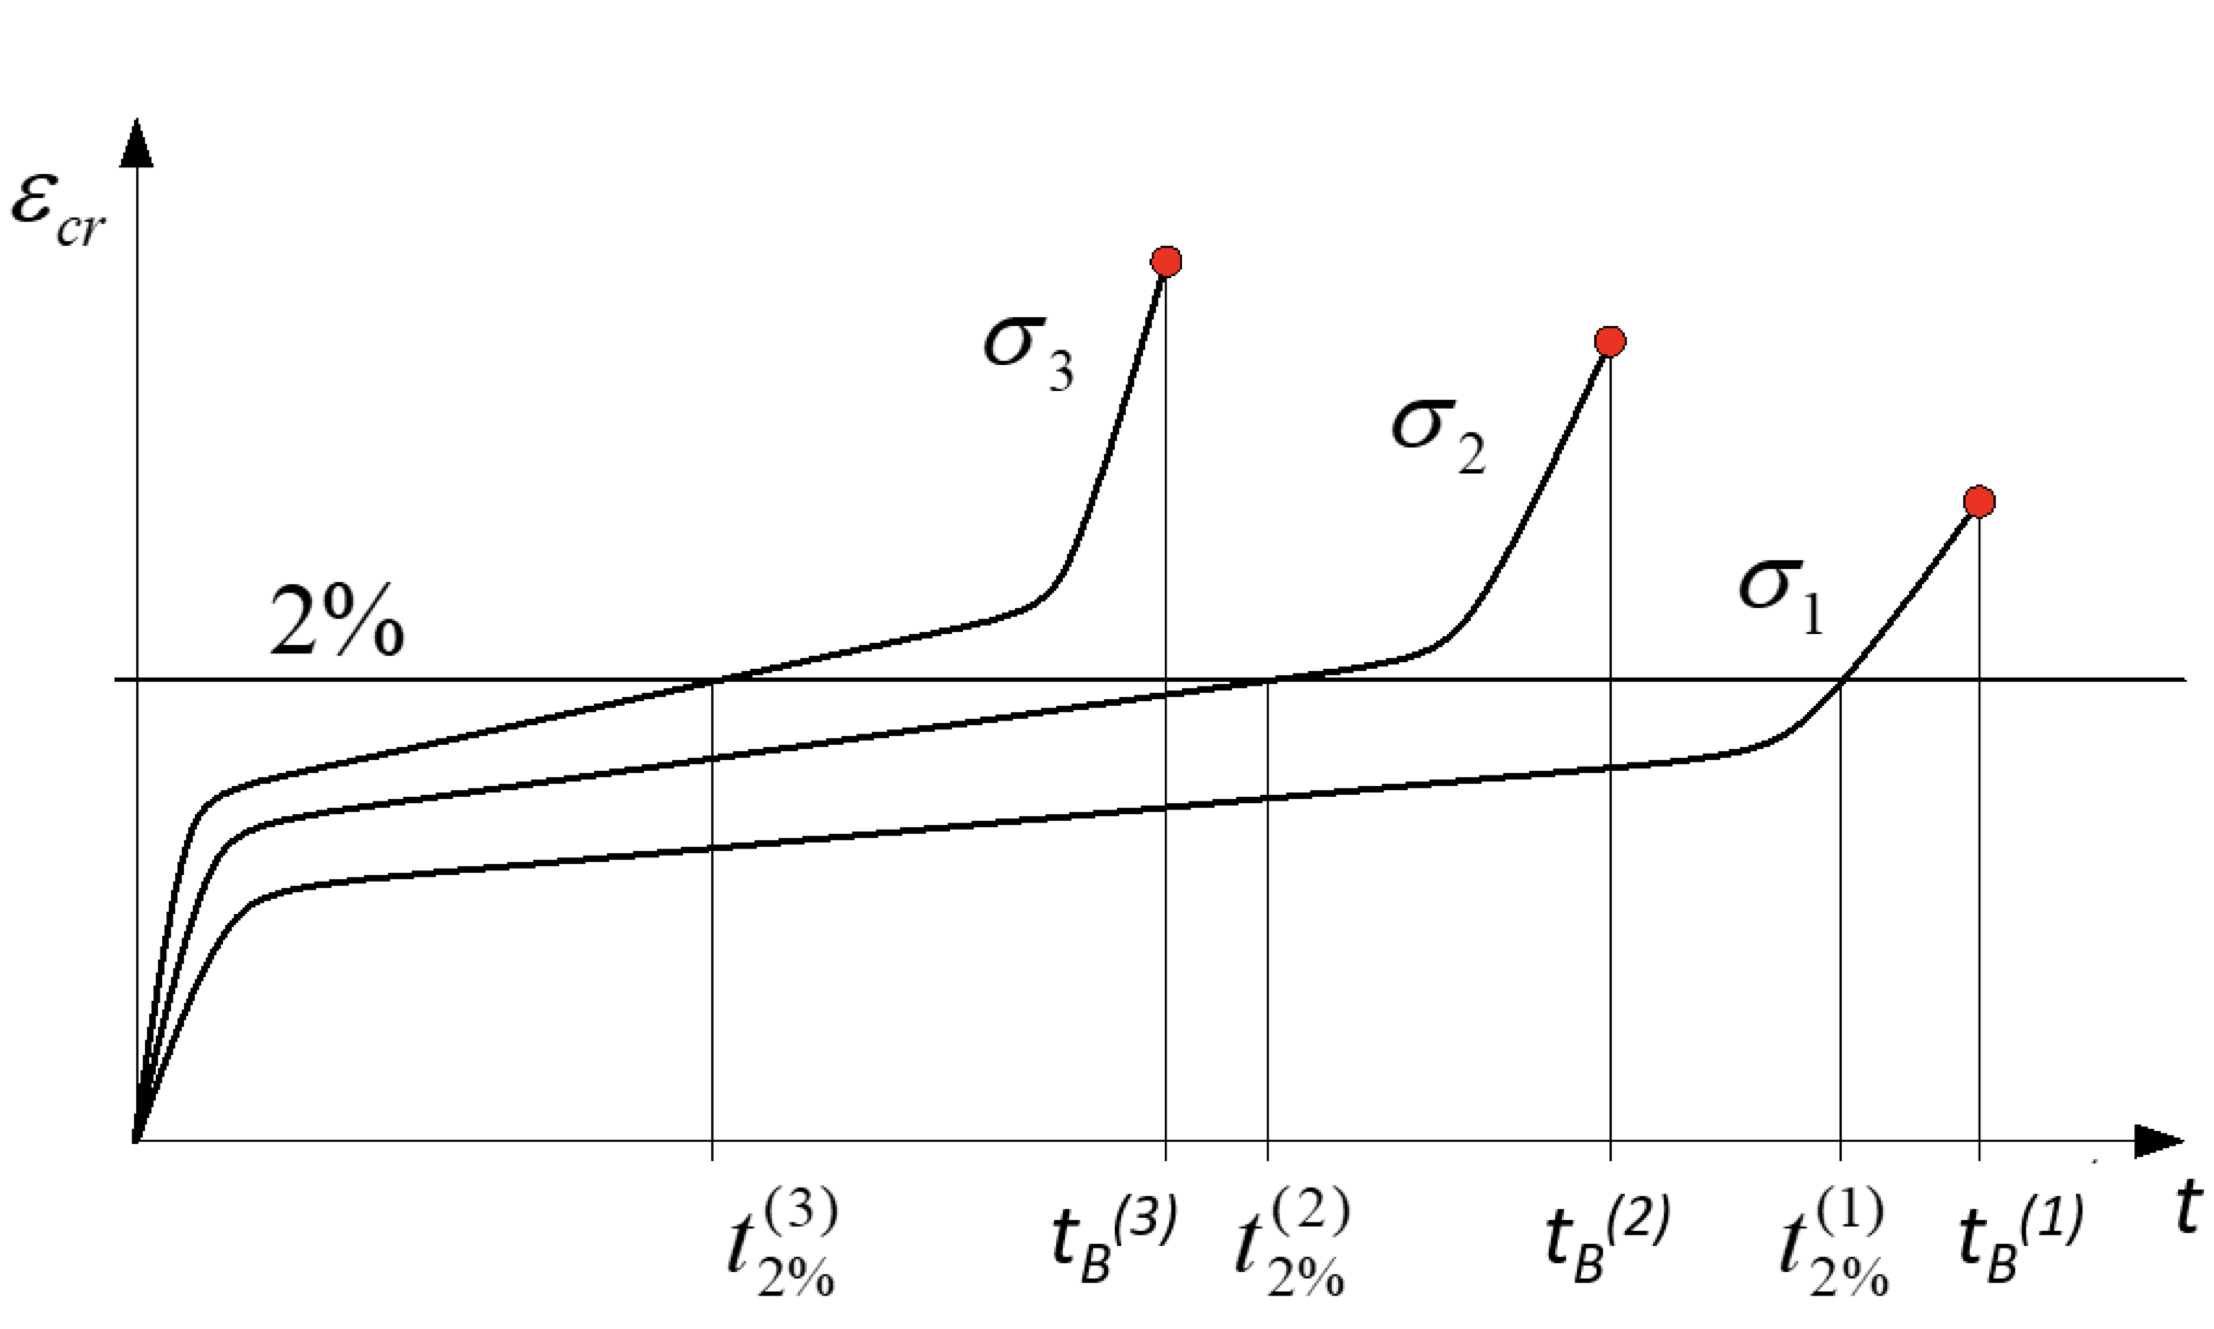
\includegraphics[width=0.55\linewidth]{08/E_cr-t-diag.png}
    \subsection{Ursachen}
        Kriechen tritt bei metallischen Stoffen bei $ T < T_{schmelz} \cdot 0.3  $ auf.
        Bewegung von Versetzungen, Gleit- und Diffussionsphänomene. $\rightarrow$ inelastische Deformation  
        
    \subsection{Relaxation}
        \subsubsection{Nach Norton}
            ges: $\sigma(t)$ geg: $\varepsilon_{cr}$, $\varepsilon{el}$
            \[\varepsilon_{cr}+\varepsilon_{el}=\varepsilon_0=\textrm{const.} \qquad \dot{\varepsilon}_{cr}+\dot{\varepsilon}_{el}=0 \Rightarrow A\sigma^n + \frac{\dot{\sigma}}{E}=0\]
            Separation der Variablen und Integrationskonstante mit Anfangsspannung bestimmen.
            \\\textbf{Analytische Lösung:}
            \[\sigma(t)=\left(\sigma_{0}^{1-n}-(1-n)A\cdot E\cdot t\right)^{\frac{1}{1-n}}\]
    \subsection{Kriechschädigung}
        \subsubsection{Kumulative Schädigung/ Time Fraction Rule}
            Aufteilen der Spannungsgeschichte $\sigma(t)$ in \textbf{diskrete Intervalle} $\Delta t_n$ mit konstanter Spannung $\sigma_n$ \& zugehöriger Rupture-Time $t_B(\sigma_n)$.
            \[D_{cr}=\sum_n\frac{\Delta T_{n}}{t_B(\sigma_n)} < 1\]
            \textbf{kontinuierliche Sannungsgeschichte:}
            \[D_{cr}=\int_0^t\frac{1}{t_B(\sigma(t))}dt < 1\]
            Spannungsrelaxation$\rightarrow \sigma(t)$ mit $\dot{\sigma}<0$
        \subsubsection{Ductility Exhaustion Method}
            \[D_{cr}=\int_0^{\bar{\varepsilon}_{cr}}\frac{1}{\varepsilon_{cr}^B(\dot{\varepsilon}_{cr})}d\varepsilon_{cr}< 1\]
            $\bar{\varepsilon}_{cr}$: ersetzen durch $\varepsilon_{cr}(t_1)$ \& $d\varepsilon_{cr} \Rightarrow \dot{\varepsilon}_{cr}dt$
            \\Beobachtung: $\varepsilon_{cr}^{B}\downarrow$ mit zunehmender Hydrostatischer Belast.
        \subsubsection{Lebensdauer}
            \[N\cdot D_{cr}^{BK} = 1\]
            $N$: Anzahl Zyklen bis zu Versagen (siehe Miner Regel)
    \subsection{Interaktion Kriechen-Ermüdung}
        Kriechen oder Relaxation innerhalb einer zyklischen Belastung führen zu niedriger $N_{zul}$ für gleiche Dehnungsschwingbreite $\Delta\varepsilon$.
        \\$D_{cr}\uparrow \quad\rightarrow\quad N_{zul}(\Delta\varepsilon)\downarrow$\\
            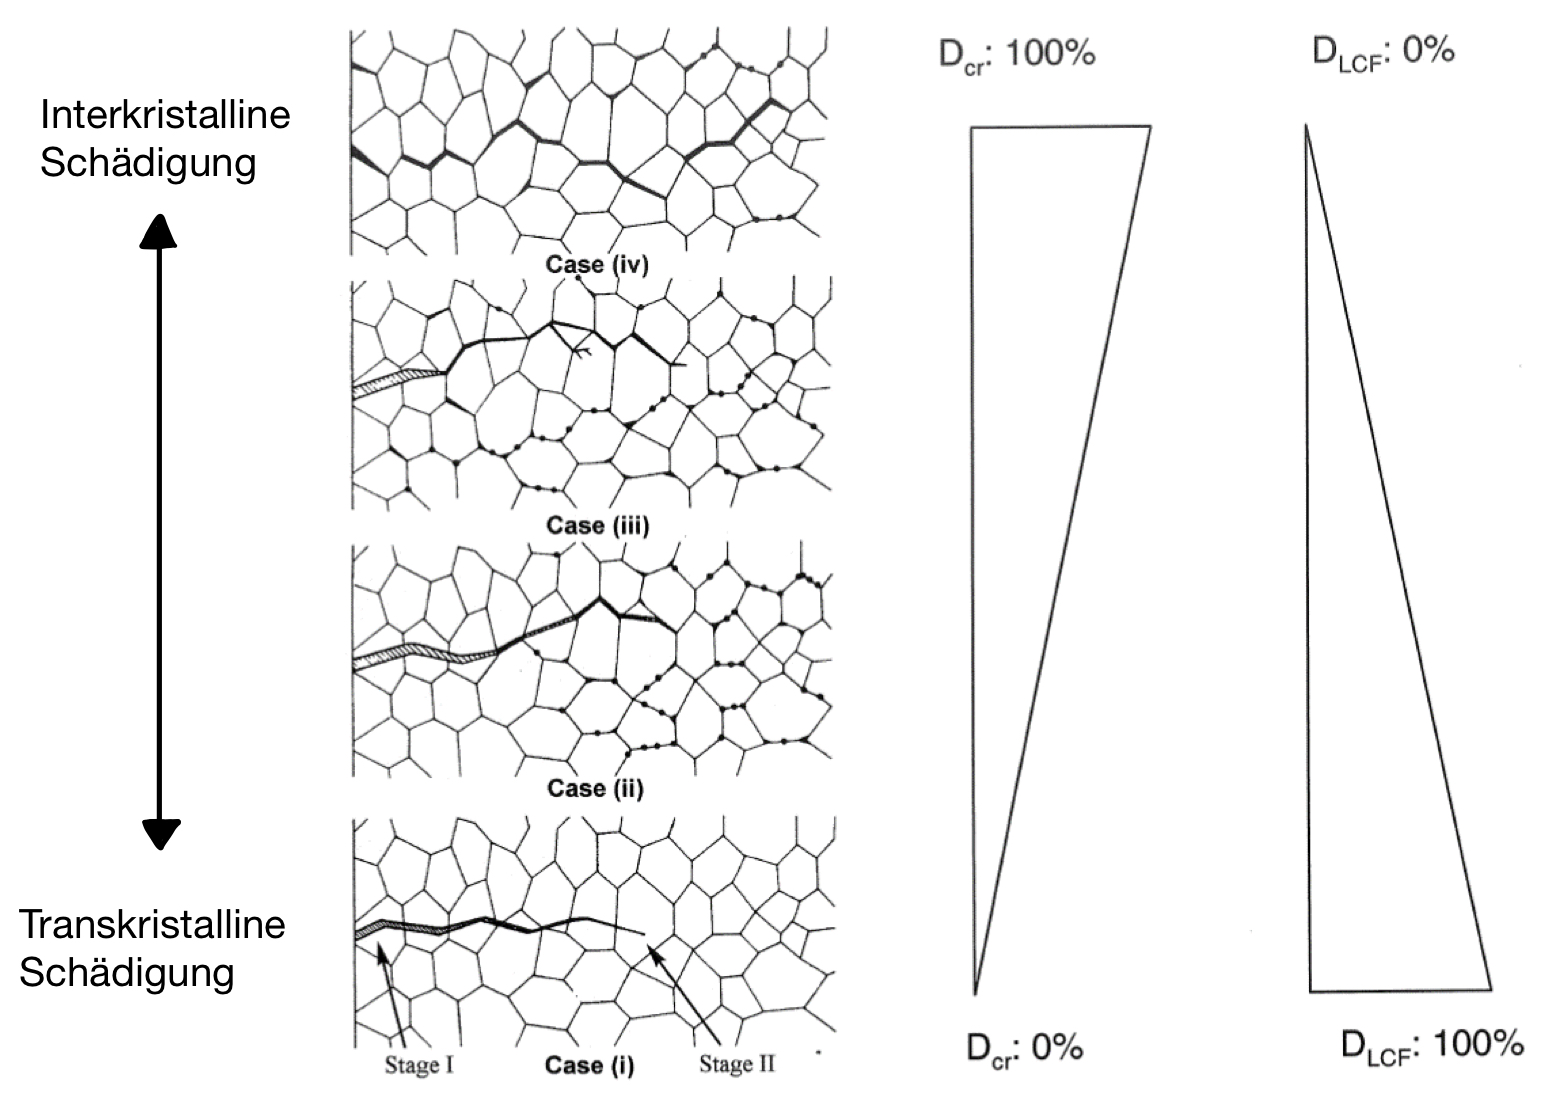
\includegraphics[width=0.55\linewidth, height=30mm]{08/LCF_schaed.jpg}
            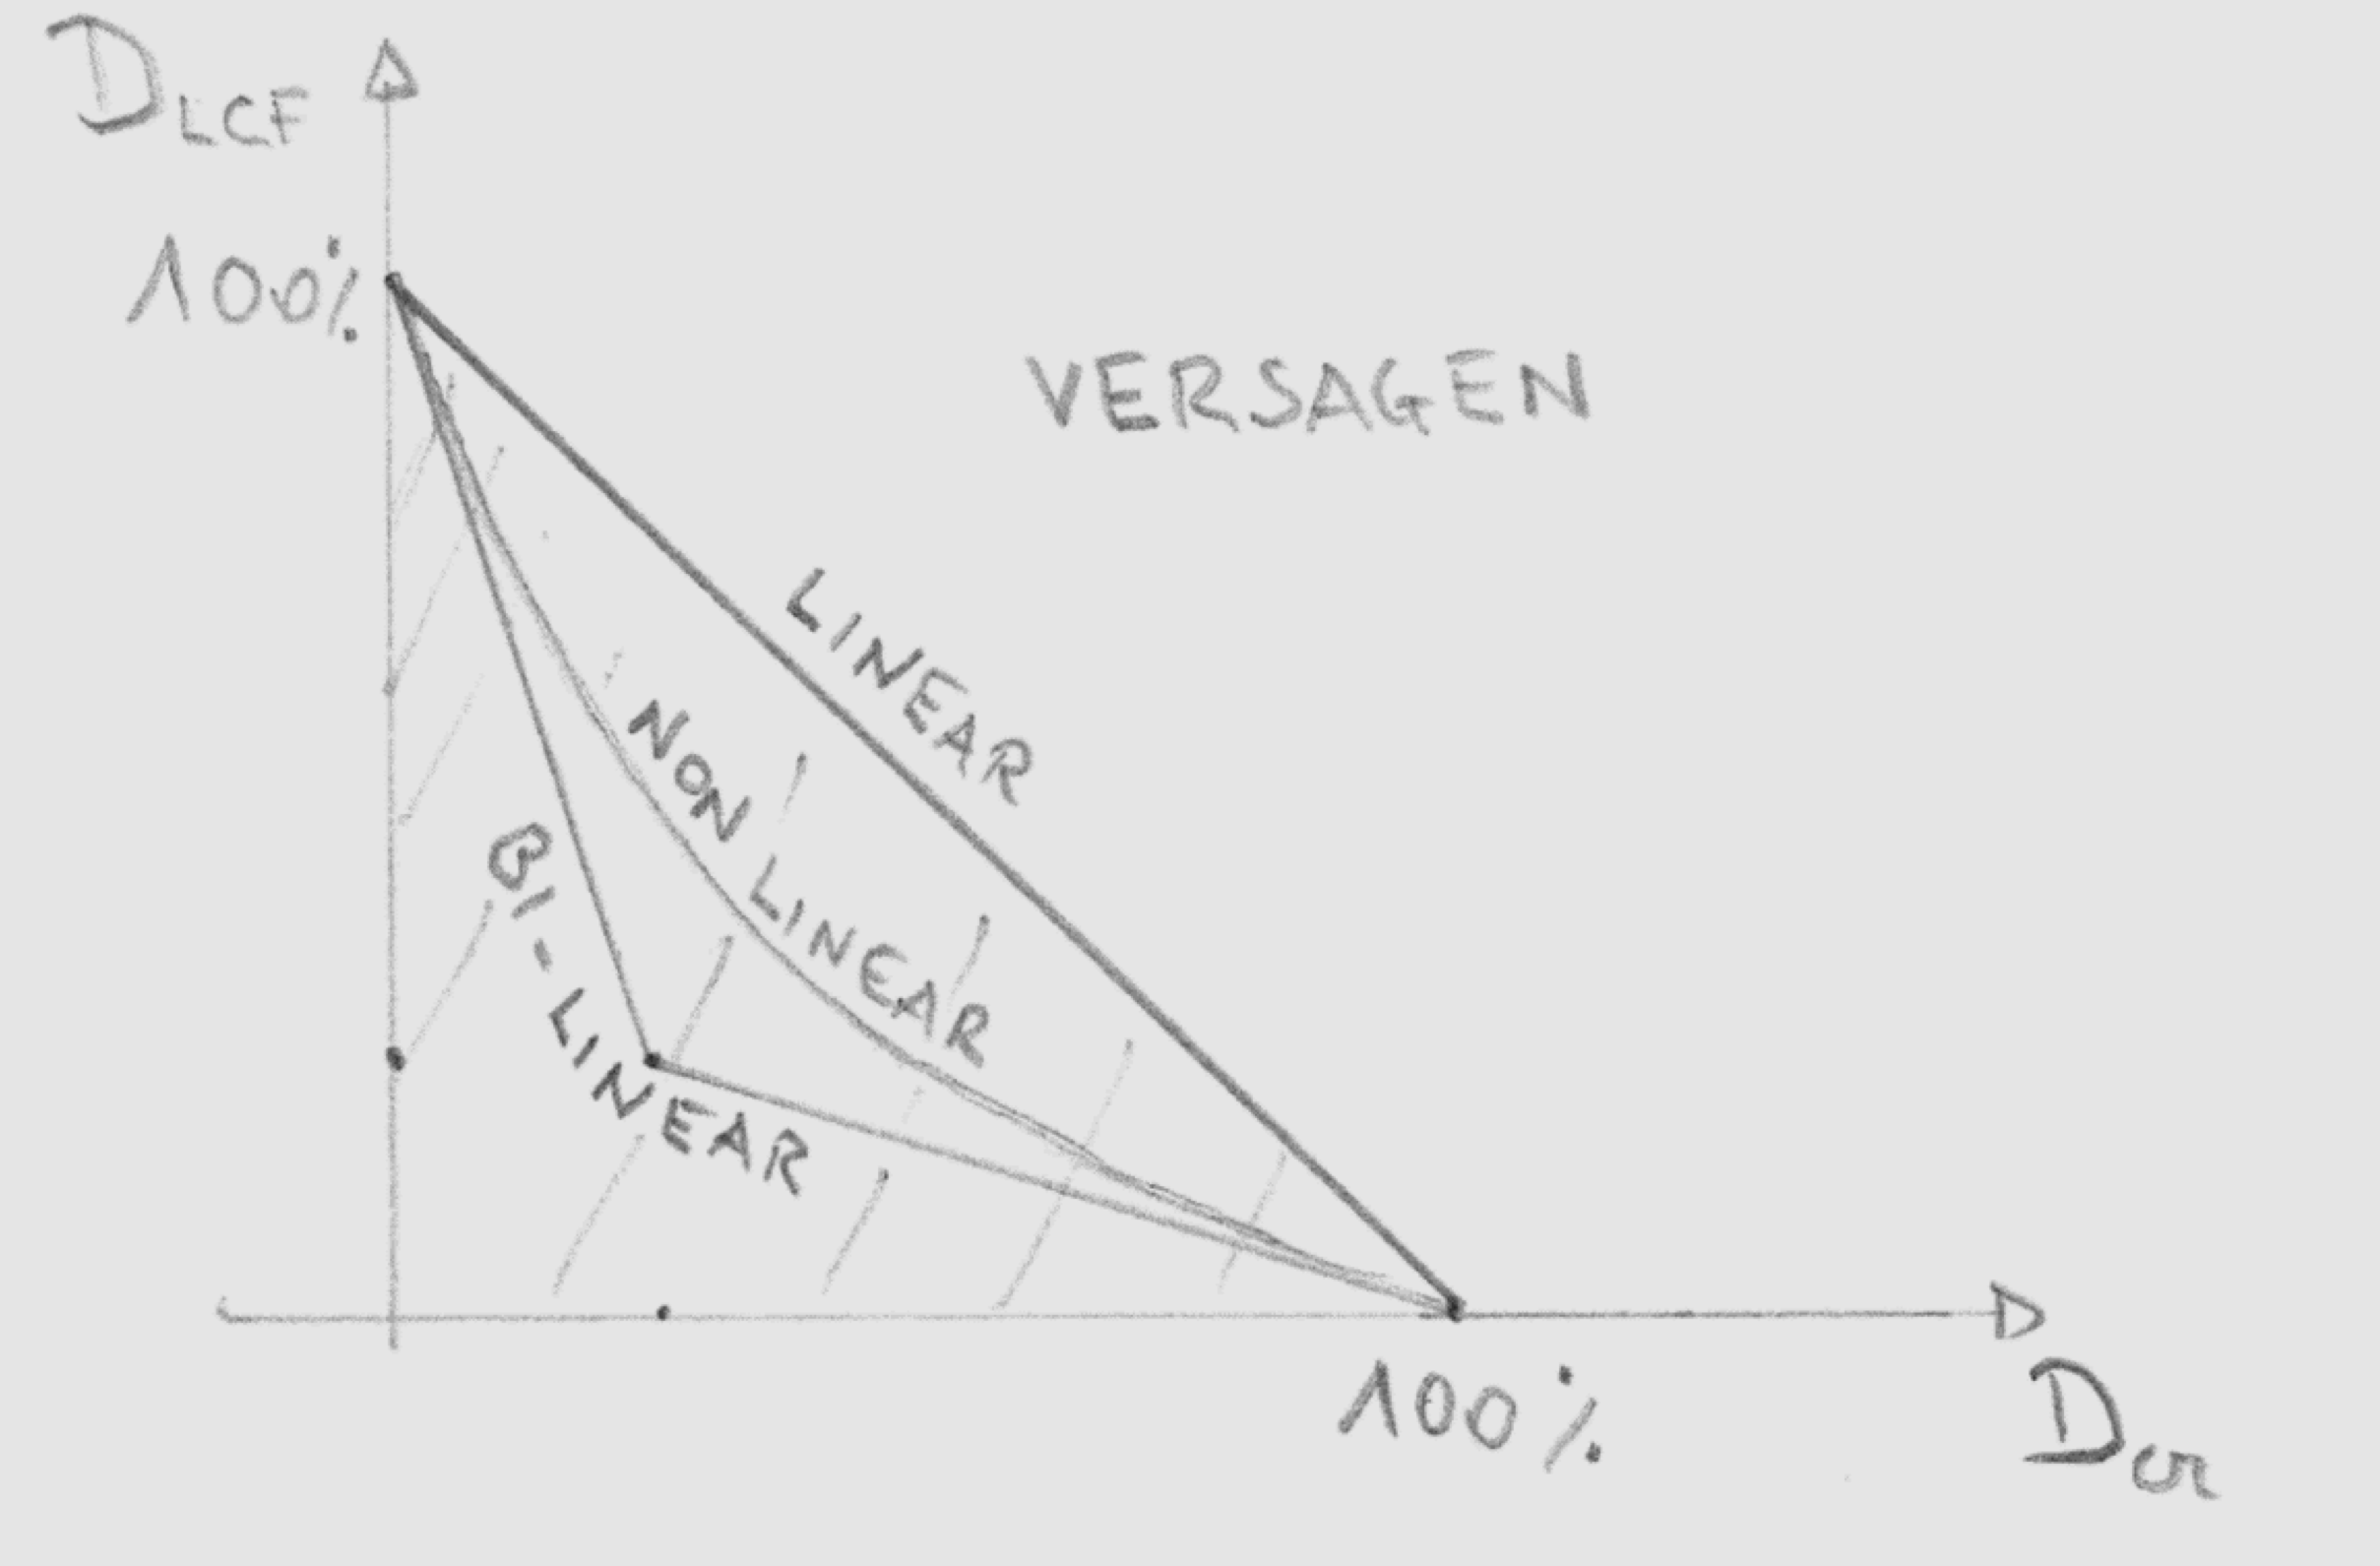
\includegraphics[width=0.45\linewidth, height=30mm]{08/damage_sum_diag.png}
        